\section{引导程序实现}\label{sec:BootloaderImplementation}

在本节(\cref{sec:BootloaderImplementation})中,笔者将详细讨论引导程序的实现,包括其定义、功能和操作系统引导过程的关键组成部分。引导加载器是启动操作系统的核心组件,它负责加载操作系统内核到内存并启动执行。整个引导过程在Rust语言的支持下,增强了系统的安全性和可靠性,通过精心设计的内存操作和错误管理,确保了引导过程的稳定性和效率。

\subsection{引导过程概述}

引导加载器(Bootloader)是一种专门用于启动操作系统的程序。其主要职责是将操作系统的内核加载到内存中并执行。在此之前,引导加载器需要完成一系列准备工作,包括将CPU从16位实模式切换到32位保护模式,并对内存段进行配置。市场上存在多种成熟的引导加载器,例如GRUB,这类引导加载器能够启动Linux、Windows等复杂的操作系统。

但本项目采用了自制的引导加载器,全部使用Rust语言编写。本项目设计的引导加载器分为两个阶段。第一阶段的引导加载器由于必须适配磁盘的第一个扇区,因此在内存容量上极为受限。它的唯一目的是为了加载第二阶段的引导加载器。第一阶段的引导加载器功能简单,仅包含启动计算机和从磁盘读取第二阶段引导加载器所需的基本代码。一旦第一阶段的任务完成,控制权就会转交给第二阶段的引导加载器,后者负责更为复杂的任务,包括初始化额外的硬件设备、设置内存管理系统、将操作系统内核加载到内存中,并最终将控制权移交给内核。

这种分阶段的启动方式大大简化了各个阶段的职责,使每个部分都能集中处理其核心功能,避免过度复杂化。此外,采用Rust语言编写引导加载器增强了系统的安全性和可靠性。Rust语言内置的内存安全特性可以有效减少常见的内存错误,为整个引导过程提供了坚实的保障。

\subsection{第一阶段引导:实模式}

\subsubsection{主引导记录(Master Boot Record,MBR)}

主引导记录(MBR)是磁盘的第一个扇区(通常是扇区0),也被称为启动扇区,因为它包含了启动操作系统所需的引导程序(通常是引导加载程序的第一阶段),大小为512字节。MBR的结构(\cref{tab:MBRStructure})包括以下几个主要部分:

\begin{enumerate}
    \item \textbf{MBR 引导代码(Boot Code,0x000-0x1B7)}:包含用于启动计算机的基本输入输出系统(BIOS)的引导代码。在计算机启动时,BIOS 会加载并执行这段代码,这是启动序列的一部分。
    \item \textbf{磁盘唯一标识符(Disk Signature,0x1B8-0x1BB)}:用于存储磁盘的唯一标识符,这有助于操作系统识别和区分不同的磁盘。
    \item \textbf{保留区域(Reserved Area,0x1BC-0x1BD)}:通常未使用,保留供将来使用。
    \item \textbf{分区表条目(Partition Entries,0x1BE-0x1FD)}:存储关于硬盘上不同分区的信息,如起始地址、分区类型、分区大小等。每个分区表条目可以定义一个主分区或扩展分区。
    \item \textbf{标志性签名(Signature, 0x1FE-0x1FF)}:最后两个字节固定为 0x55AA,这是用来识别有效的引导扇区的标志。
\end{enumerate}

\begin{longtable}[c]{@{}ccc@{}}
    \caption{MBR结构}
    \label{tab:MBRStructure}                       \\
    \toprule
    \textbf{偏移量} & \textbf{大小 (字节)} & \textbf{描述}  \\ \midrule
    \endfirsthead
    \multicolumn{3}{r}{\textbf{续表~\thetable}}      \\
    \toprule
    \textbf{偏移量} & \textbf{大小 (字节)} & \textbf{描述}  \\ \midrule
    \endhead
    \hline
    \multicolumn{3}{r}{续下页}
    \endfoot
    \endlastfoot
    0x000        & 440              & MBR 引导代码     \\
    0x1B8        & 4                & 磁盘唯一标识符      \\
    0x1BC        & 2                & 保留区域         \\
    0x1BE        & 16               & 分区表条目        \\
    0x1CE        & 16               & 分区表条目        \\
    0x1DE        & 16               & 分区表条目        \\
    0x1EE        & 16               & 分区表条目        \\
    0x1FE        & 2                & 标志性签名 0x55AA \\ \bottomrule
\end{longtable}

当从磁盘引导时,BIOS自动将该磁盘的第一个扇区加载到内存地址0x7C00,并跳转到该地址执行MBR引导程序。

在MinmusOS中,MBR引导程序是引导加载器的第一阶段。这是一个极其受限的环境,因为必须只有440字节的程序能够将引导加载器的第二阶段加载到内存中并执行它。因此,这部分引导程序通常使用汇编语言编写,以实现尽可能的优化。然而,Rust编译器也能生成优化的二进制文件,使其适用于此目的。因此,MinmusOS的第一阶段引导程序主要用Rust编写,除了一小部分用汇编编写的程序,负责:

\begin{enumerate}
    \item 禁用硬件中断
    \item 将数据段寄存器置零
    \item 设置堆栈
    \item 调用Rust主函数
\end{enumerate}

这样的设计充分利用了Rust的性能优势,同时保留汇编语言处理底层硬件操作的能力。

\subsubsection{BIOS 中断(BIOS Interrupts)}

在引导加载器的第一阶段,由于内存环境非常受限,它无法实现自己的磁盘驱动程序。因此,引导加载器使用 BIOS 中断来访问硬件,执行各种任务,如在屏幕上打印信息或从磁盘读取数据。

BIOS 中断调用是由 BIOS 提供的函数,用于简化和抽象硬件访问。这些中断调用只能在 16 位实模式下工作,因此它们不适合作为硬件驱动程序,而仅用于在启动过程中帮助引导加载器工作。当 CPU 进入 32 位保护模式时,BIOS 中断就无法工作,因此内核必须实现自定义硬件驱动程序。

MinmusOS 的引导加载器使用 BIOS 中断 0x13 从磁盘读取数据。这个中断要求设置一个磁盘地址包(Disk Address Packet,DAP)结构,用于指定要读取的扇区数、逻辑块地址(LBA),以及将数据写入内存的位置。数据结构定义如\cref{lst:DiskAddressPacketDataStructure}所示:

\begin{listing}[htbp]
    \begin{minted}{rust}
#[repr(C, packed)]
struct DiskAddressPacket {
    size: u8,
    zero: u8,
    sectors: u16,
    offset: u16,
    segment: u16,
    lba: u64,
}
    \end{minted}
    \caption{DiskAddressPacket数据结构定义}\label{lst:DiskAddressPacketDataStructure}
\end{listing}

\begin{enumerate}
    \item \texttt{size}:表示这个结构体的大小(以字节为单位)。用来向 BIOS 提供这个结构体大小的信息,确保 BIOS 正确解释剩余的字段。
    \item \texttt{zero}:这个字段通常设置为0,用于填充或确保结构体的对齐。
    \item \texttt{sectors}:指定要读取的扇区数量。因为 BIOS 中断 0x13 是以扇区为单位进行数据传输的,这个字段告诉 BIOS 一次操作需要读取多少扇区。
    \item \texttt{offset}:数据应该被加载到的内存段内的偏移地址。这告诉 BIOS 从磁盘读取数据后,数据应该存储在哪个具体的内存位置。
    \item \texttt{segment}:这是内存段的地址,与 offset 一起决定数据最终存放的物理内存位置。在实模式下,物理地址计算公式是 $segment \times 16 + offset$。
    \item \texttt{lba}:逻辑块寻址(Logical Block Addressing,LBA)的起始地址。这是一个64位的值,用来指定从哪个扇区开始读取数据。LBA 模式允许以线性方式访问硬盘上的扇区,而不需要考虑物理磁盘的几何结构(如柱面、磁头、扇区)。
\end{enumerate}

这个结构的打包(packed)属性是必须的,因为它确保编译器不会在成员之间插入填充,从而满足 BIOS 对于这种结构数据严格的内存布局要求。这是在低级系统编程中常见的做法,用以确保与硬件之间的接口按预期工作。

在发出中断之前,引导加载器需要设置一些 CPU 寄存器:

\begin{enumerate}
    \item \textbf{DS:SI}:设置为 DAP(磁盘地址包)的地址。DS 是段寄存器,SI 是偏移量寄存器,二者组合提供了数据结构的完整物理地址。
    \item \textbf{AH}:设置为 0x42。在 INT 0x13 的多个功能中,AH=0x42 对应于扩展读盘操作,它支持使用逻辑块地址(LBA)而非传统的柱面-磁头-扇区(CHS)寻址方式。
    \item \textbf{DL}:设置为驱动器号(对于主驱动器是 0x80)。DL 寄存器指定了要访问的磁盘驱动器号。
\end{enumerate}

然后发出 INT 0x13 中断将调用 BIOS 函数,从磁盘读取数据。如果在读取过程中发生错误,进位标志(carry flag)\footnote{进位标志(Carry Flag):这是 CPU 状态寄存器中的一位,用来指示上一个算术或逻辑操作是否产生了进位或借位。在使用 INT 0x13 时,如果操作成功,进位标志将被清除(设置为 0);如果操作失败,进位标志将被设置(设置为 1)。}将会被设置。MinmusOS 的引导加载器使用 JC 指令\footnote{JC(Jump if Carry)指令:这是一个条件跳转指令,只有在进位标志为 1 时才执行跳转。在引导加载器中,如果 INT 0x13 调用失败,进位标志会被设置,JC 指令将跳转到错误处理代码,通常会显示错误信息或停止进一步执行。}来检查这个标志,并通知用户错误发生。

另一个 BIOS 中断是 INT 0x10,INT 0x10 是一个 BIOS 提供的视频服务中断。这个中断提供了多种与显示相关的功能,如设置显示模式、更改字符颜色、移动光标以及打印字符到屏幕等,它在引导加载器中被用来打印字符串到屏幕上。然而,这个中断只在引导加载器中使用,因为内核实现了一个更复杂的打印功能,该功能直接写入到视频内存。

\subsubsection{启动模块(Boot Module)}

这个模块包括一个 Assembly 文件和其 Rust 接口的集成,负责禁用硬件中断,将数据段寄存器置零,设置堆栈,并且跳转到 Rust 主程序。

\begin{listing}[htbp]
    \begin{minted}{asm}
.section .boot, "awx"
.global _start
.code16

_start:
    cli

    xor ax, ax
    mov ds, ax
    mov es, ax
    mov ss, ax
    mov fs, ax
    mov gs, ax

    cld
    mov sp, 0x7c00

    call main

spin:
    hlt
    jmp spin
    \end{minted}
    \caption{boot/src/boot.asm}\label{lst:BootASM}
\end{listing}

这段汇编代码(\cref{lst:BootASM})是用于启动操作系统的Master Boot Record(MBR)的引导程序的一部分,位于硬盘的最开始的扇区。详细解释如下:

\begin{enumerate}
    \item \textbf{节和全局设置}
          \begin{enumerate}
              \item \texttt{.section .boot, "awx"}:定义一个名为 .boot 的段,属性为“awx”,表示该段是可分配的、可写的以及可执行的。
              \item \texttt{.global \_start}:定义 \_start 标签为全局,使得链接器可以找到它作为程序的入口点。
              \item \texttt{.code16}:指定代码为 16 位模式,适用于 BIOS 在实模式下工作。
          \end{enumerate}
    \item \textbf{禁用外部中断}
          \begin{enumerate}
              \item \texttt{cli}:Clear Interrupt Flag,清除中断标志,禁用硬件中断,确保在初始化过程中不会被外部事件打断。
          \end{enumerate}
    \item \textbf{设置数据段寄存器为零}
          \begin{enumerate}
              \item \texttt{xor ax, ax}:将 AX 寄存器清零。AX 寄存器是 x86 架构处理器中的一个通用寄存器,它是一个 16 位的寄存器,可以用于存储数据、执行算术和逻辑操作等。
              \item \texttt{mov ds, ax}等:将所有数据段寄存器(DS、ES、SS、FS、GS)设置为 0,初始化段寄存器,为后续程序的运行提供干净的段环境。
          \end{enumerate}
    \item \textbf{设置栈指针}
          \begin{enumerate}
              \item \texttt{cld}:Clear Direction Flag,清除方向标志,确保字符串操作在内存中从低地址向高地址移动。
              \item \texttt{mov sp, 0x7c00}:设置栈指针 SP 到 0x7c00,这是 BIOS 加载 MBR 程序的起始地址。由于栈是向下增长的,所以初始化栈指针到程序加载的起始地址是为了确保栈空间不会与程序空间冲突。
          \end{enumerate}
    \item \textbf{调用Rust主函数}
          \begin{enumerate}
              \item \texttt{call main}:调用标签为 main 的函数,这是用 Rust 编写的主函数,用于执行更复杂的任务。
          \end{enumerate}
    \item \textbf{防止程序执行溢出}
          \begin{enumerate}
              \item \texttt{hlt}:Halt 指令用于停止 CPU 的执行直到下一个外部中断被触发。
              \item \texttt{jmp spin}:无限循环,确保如果 main 函数返回,CPU 不会执行任何未定义的操作或跑到程序代码以外的地方去。
          \end{enumerate}
\end{enumerate}

在完成了启动模块的基础设置和功能调用之后,系统的硬件环境和内存状态被适当配置和初始化,为主启动程序的加载和执行提供了必要的条件。此时,CPU仍处于16位实模式,限制了对现代硬件特性的全面控制和访问。接下来,控制权将被传递到主启动程序,这一程序将负责进一步的系统启动过程,包括引导更复杂的操作系统核心组件。

\subsubsection{磁盘读取器模块(Disk Reader Module)}

这个模块负责从磁盘读取数据。它定义了 DiskReader 结构和相关方法,使用 BIOS 中断 0x13 来进行实际的磁盘操作。该模块使用了线性块地址(LBA)方式而不是传统的柱面-磁头-扇区(CHS)方式,这是现代磁盘访问的常用方法。这里使用的是一种称为磁盘地址包(Disk Address Packet,DAP)的数据结构(见\cref{lst:DiskAddressPacketDataStructure}),以支持这种访问方式。

DiskReader 结构体(\cref{lst:DiskReaderDataStructure})用于封装磁盘读取操作的状态,包括:

\begin{enumerate}
    \item \texttt{lba}:起始线性块地址
    \item \texttt{target}:数据应该加载到的内存地址
\end{enumerate}

\begin{listing}[htbp]
    \begin{minted}{rust}
pub struct DiskReader {
    lba: u64,
    target: u16,
}
    \end{minted}
    \caption{DiskReader数据结构定义}\label{lst:DiskReaderDataStructure}
\end{listing}

\paragraph{方法 \texttt{new(lba: u64, target: u16) -> Self}}

这个 new 方法是 DiskReader 结构体的构造函数,用于创建 DiskReader 实例。它接受两个参数:lba 和 target。lba 参数是一个 u64 类型的值,代表线性块地址,用来指定从哪个扇区开始读取数据。这允许构造函数支持大容量存储设备上的磁盘操作。target 参数是一个 u16 类型的值,表示数据加载到内存中的目标偏移地址。

通过这个构造函数,用户可以方便地创建一个配置好的 DiskReader 实例,随后可用于执行磁盘读取操作。这个设计简洁而有效,确保了 DiskReader 在创建时就被正确地配置。

\paragraph{方法 \texttt{read\_sector()}}

read\_sector 方法(\cref{lst:ReadSectorMethod})的主要功能是读取从特定线性块地址(LBA)开始的一个扇区的数据,并将数据存储到指定的内存偏移地址。该方法使用 DiskAddressPacket 结构体来配置读取操作的细节,并通过 INT 0x13 BIOS 中断进行磁盘访问。

\begin{listing}[htbp]
    \begin{minted}{rust}
pub fn read_sector(&self) {
    let dap = DiskAddressPacket {
        size: size_of::<DiskAddressPacket>() as u8,
        zero: 0,
        sectors: 1,
        offset: self.target,
        segment: 0x0000,
        lba: self.lba,
    };

    let dap_address = &dap as *const DiskAddressPacket;

    unsafe {
        core::arch::asm!(
        "mov {1:x}, si",
        "mov si, {0:x}",
        "int 0x13",
        "jc fail",
        "mov si, {1:x}",
        in(reg) dap_address as u16,
        out(reg) _,
        in("ax") 0x4200u16,
        in("dx") 0x0080u16,
        );
    }
}
    \end{minted}
    \caption{\texttt{read\_sector()}方法}\label{lst:ReadSectorMethod}
\end{listing}

在这个方法中,首先创建了一个 DiskAddressPacket 的实例 dap,具体字段配置如下:

\begin{enumerate}
    \item \texttt{size}:结构体的大小,使用 \texttt{size\_of::<DiskAddressPacket>()} 动态获取,保证与实际定义匹配。
    \item \texttt{zero}:固定为0,作为填充字段。
    \item \texttt{sectors}:设置为1,表示此次操作只读取一个扇区。
    \item \texttt{offset}和\texttt{segment}:指定数据加载到内存中的位置。offset 为 self.target,是调用时指定的内存地址偏移;segment 设置为 0x0000,通常是在实模式下使用的段基址。
    \item \texttt{lba}:从该线性块地址读取数据,对应于 DiskReader 实例中存储的 lba 字段。
\end{enumerate}

在 DiskAddressPacket 配置完成后,代码获取这个结构体的地址 dap\_address,然后通过内联汇编进行以下操作:

\begin{enumerate}
    \item \textbf{保存和设置寄存器}
          \begin{enumerate}
              \item \texttt{mov {1:x}, si}:保存原始 si 寄存器的值,以便恢复。
              \item \texttt{mov si, {0:x}}:将 DiskAddressPacket 的地址放入 si 寄存器,因为 INT 0x13 需要通过 si 传递参数。
          \end{enumerate}
    \item \textbf{执行 BIOS 中断}
          \begin{enumerate}
              \item \texttt{int 0x13}:执行磁盘读操作。ax 寄存器设置为 0x4200,表示执行读操作;dx 设置为 0x0080,表示第一个硬盘。
          \end{enumerate}
    \item \textbf{错误检查}
          \begin{enumerate}
              \item \texttt{jc fail}:如果操作失败(进位标志被设置),则跳转到错误处理标签 fail(需要在代码中定义该标签的行为)。
          \end{enumerate}
    \item \textbf{恢复寄存器}
          \begin{enumerate}
              \item \texttt{mov si, {1:x}}:恢复 si 寄存器的原始值。
          \end{enumerate}
\end{enumerate}

这种方式直接使用 BIOS 提供的功能来访问硬件,允许在没有操作系统支持的环境下(如引导加载器)进行低层次的磁盘操作。通过这个方法,DiskReader 可以读取磁盘上特定位置的数据,对于操作系统的启动和运行至关重要。

\paragraph{方法 \texttt{read\_sectors(sectors: u16)}}

该 read\_sectors 方法(\cref{lst:ReadSectorsBootMethod})是 DiskReader 结构体的成员方法,其功能是读取多个连续的扇区数据。方法接受一个参数 sectors,表示需要读取的扇区数量。该方法通过循环调用 read\_sector 方法来逐一读取指定数量的扇区,并适当更新目标内存地址和LBA地址。

\begin{listing}[htbp]
    \begin{minted}{rust}
pub fn read_sectors(&mut self, sectors: u16) {
    let mut sectors_left = sectors;
    while sectors_left > 0 {
        self.read_sector();
        self.target += SECTOR_SIZE;
        self.lba += 1;
        sectors_left -= 1;
    }
}
    \end{minted}
    \caption{\texttt{read\_sectors(sectors: u16)}方法}\label{lst:ReadSectorsBootMethod}
\end{listing}

以下是对该方法的解释:

\begin{enumerate}
    \item \textbf{初始化计数器}:创建一个变量 sectors\_left 用于追踪还剩多少扇区需要读取。
    \item \textbf{循环读取扇区}:使用一个循环来连续读取扇区,直到 sectors\_left 减到0,这意味着所有指定的扇区都已经读取完成。
    \item \textbf{读取单个扇区}:调用 read\_sector 方法读取一个扇区的数据。
    \item \textbf{更新内存地址和LBA地址}:每读取一个扇区后,将目标内存地址向前移动一个扇区的大小(512字节),这样下一个扇区的数据就不会覆盖前一个扇区的数据;将LBA地址递增1,以便下一次读取操作定位到下一个扇区。
    \item \textbf{递减剩余扇区计数}:每次循环结束后,将剩余扇区数减1。
\end{enumerate}

这个方法通过更新内存偏移地址和LBA地址,使得可以连续地读取多个扇区到指定的内存区域中。

\subsubsection{主启动程序(Main Boot Program)}\label{sec:MainBootProgram}

这个模块(\cref{lst:BootSrcMain})是系统的主入口,使用 Rust 编写。它负责加载并执行 bootloader,并处理初始化中的错误。

\begin{listing}[htbp]
    \begin{minted}{rust}
#![no_std]
#![no_main]

...

const BOOTLOADER_LBA: u64 = 2048;
const BOOTLOADER_SIZE: u16 = 64;

global_asm!(include_str!("boot.asm"));

extern "C" { static _bootloader_start: u16; }

#[no_mangle]
pub extern "C" fn main() -> ! {
    unsafe { asm!("mov ah, 0x00", "mov al, 0x03", "int 0x10"); }
    print("[INFO] Booting MinmusOS...\r\n\0");
    print("[INFO] Loading Bootloader...\r\n\0");
    let bootloader_start: *const u16 = unsafe { &_bootloader_start };
    let target = bootloader_start as u16;
    let mut disk = DiskReader::new(BOOTLOADER_LBA, target);
    disk.read_sectors(BOOTLOADER_SIZE);
    unsafe { asm!("jmp {0:x}", in(reg) bootloader_start as u16); }
    loop {}
}

fn print(message: &str) {
    unsafe {
        asm!(
        "mov si, {0:x}", // 将 message 的地址加载到 SI 寄存器
        "2:",            // 标签 2,这是一个循环的开始点
        "lodsb",         // 从 SI 指向的地址加载一个字节到 AL 寄存器,并将 SI 自增
        "or al, al",     // 将 AL 寄存器的内容与其自身进行 OR 操作,主要用来设置零标志(ZF)
        "jz 3f",         // 如果结果为零(即 AL 为零,表明字符串结束),则跳转到标签 3
        "mov ah, 0x0e",  // 将 0x0E 加载到 AH 寄存器,设置 BIOS 的 teletype 输出
        "mov bh, 0",     // 将显示页面设置为 0,通常用于多页面管理
        "out 0xe9, al",  // 输出到 0xE9 端口,这通常是用于调试的端口
        "int 0x10",      // 调用 BIOS 视频中断,使用 AH = 0x0E 和 AL 的值在屏幕上打印字符
        "jmp 2b",        // 无条件跳回到标签 2,继续循环读取下一个字符
        "3:",            // 标签 3,循环结束的地方
        in(reg) message.as_ptr(),
        );
    }
}

#[no_mangle]
pub extern "C" fn fail() -> ! {
    print("[ERROR] Failed to Load Bootloader!\r\n\0");
    loop {}
}

#[panic_handler]
fn panic(_info: &PanicInfo) -> ! { loop {} }
    \end{minted}
    \caption{boot/src/main.rs}\label{lst:BootSrcMain}
\end{listing}

\paragraph{全局和外部声明}

\texttt{\#![no\_std]}:指示编译器不使用标准库,这是操作系统和裸机程序的常见需求,因为标准库依赖于操作系统的功能。

\texttt{\#![no\_main]}:表示没有常规的 main 函数入口,这是裸机或操作系统开发中常见的设置。

\texttt{BOOTLOADER\_LBA}:定义引导加载器所在的逻辑块地址(LBA)。

\texttt{BOOTLOADER\_SIZE}:定义引导加载器大小,单位为扇区。

\texttt{global\_asm!}:插入全局汇编代码,这里包括从“boot.asm”文件中读取的汇编代码,通常用于设置初步的启动环境。

\paragraph{主入口函数 \texttt{main}}

main 函数是 MinmusOS 引导程序的核心入口点,它负责初始化系统并引导操作系统。在裸机或操作系统开发中,这个函数代替了常规应用程序中的标准 main 函数。\texttt{\#[no\_mangle]} 属性用于防止编译器修改函数名的装饰或混淆,即确保函数名在编译后保持不变。以下是对这个函数中每一步操作的详细解释:

\begin{enumerate}
    \item \textbf{设置视频模式}:\texttt{mov ah, 0x00} 和 \texttt{mov al, 0x03} 这两条指令准备寄存器 ah 和 al 以设置 BIOS 视频中断(int 0x10)的参数。ah = 0x00 代表设置视频模式的功能,al = 0x03 指定具体的视频模式,这里是标准的文本模式(80 \times 25 字符)。
    \item \textbf{打印启动信息}:调用 print 函数来在屏幕上显示启动信息,帮助用户了解当前引导进程的状态。
    \item \textbf{获取引导加载器起始地址}:通过外部链接的静态变量 \_bootloader\_start(由链接器脚本定义)获取引导加载器的起始内存地址。
    \item \textbf{初始化磁盘读取器}:将引导加载器的起始地址转换为 u16 类型,以便作为磁盘读取的目标内存地址。然后创建一个 DiskReader 实例,用于从指定的 LBA 地址开始读取数据到内存。
    \item \textbf{读取引导加载器到内存}:调用 DiskReader 的 read\_sectors 方法从磁盘读取 BOOTLOADER\_SIZE 个扇区的数据到内存中 target 指定的位置。
    \item \textbf{跳转到引导加载器执行}:使用内联汇编指令 jmp 直接跳转到引导加载器的起始地址,开始执行引导加载器的代码。
    \item \textbf{无限循环}:在正常情况下,jmp 指令后的代码不应该被执行,因为控制权已经转移给引导加载器。无限循环确保了在任何意外情况下,CPU 不会执行未定义的内存区域。
\end{enumerate}

\paragraph{打印函数 \texttt{print}}

在 MinmusOS 中的 print 函数负责将文本消息输出到屏幕,它通过 BIOS 中断 int 0x10 实现。这个函数使用内联汇编来直接与硬件交互。

\paragraph{错误处理函数 \texttt{fail}}

错误处理函数 fail 在 MinmusOS 的启动过程中加载引导加载器失败时被调用,用于显示错误信息并将系统置于无限循环状态,从而防止执行进一步的可能错误操作。

\paragraph{紧急停止处理函数 \texttt{panic}}

紧急停止处理(panic handler)是一种特殊的函数,用于处理运行时遇到的不可恢复的错误。它在程序遇到严重错误时被调用,如内存访问错误、预期之外的执行分支等。该函数的主要目的是防止程序继续执行可能危险或未定义的操作,它通过进入一个无限循环,使系统停留在已知的状态,便于调试和维护。在实际部署中,这种机制对于保持系统的稳定性和安全性至关重要,尤其是在裸机环境或操作系统的底层实现中。

\subsubsection{链接器脚本(Linker Script)}\label{LinkerScript}

链接器脚本(\cref{lst:BootLinkerScript})用于定义和控制操作系统引导程序的内存布局。脚本总体可以分为以下几个关键部分来概括其作用:

\begin{enumerate}
    \item \textbf{入口点配置}:脚本指定了程序的入口点 \_start,确保程序加载后从正确的位置开始执行。
    \item \textbf{栈配置}:脚本设置了栈的起始和结束位置,确保程序在执行时具有正确的栈空间进行操作。
    \item \textbf{段定义}:脚本详细定义了多个段,包括引导代码段 .boot,程序的主要执行代码段 .text,只读数据段 .rodata,以及包含初始化的全局变量和静态变量的数据段 .data。这些段的配置关键支持了程序数据和代码的正确加载和执行。
    \item \textbf{磁盘和分区表配置}:脚本设置了磁盘标识符和两个分区表,详细定义了启动分区和主分区的属性,这对于系统启动和磁盘管理至关重要。
    \item \textbf{魔数和引导加载器位置}:脚本的最后部分定义了引导扇区的魔数 0xAA55,保证引导扇区的有效性,同时标记了引导加载器的起始位置,确保引导过程可以正确地定位和加载引导加载器。
\end{enumerate}

整个链接器脚本确保了引导程序的内存布局和磁盘布局的准确性,对于系统的引导和加载过程至关重要。

\begin{listing}[htbp]
    \begin{minted}{text}
/* 配置程序入口点 */
ENTRY(_start)

/* 配置段的顺序和位置 */
SECTIONS {
    /* 配置栈的开始和结束位置 */
    . = 0X500;
    _stack_start = .;
    . = 0X7C00;
    _stack_end = .;

    /* 定义引导代码段,包含所有 .boot 和 .boot.* 段的内容 */
    .boot : { ... }

    /* 定义文本段,包含程序的主要执行代码 */
    .text : { ... }

    /* 定义只读数据段,包含字符串常量等不可修改的数据 */
    .rodata : { ... }

    /* 定义数据段,包含初始化的全局变量和静态变量 */
    .data : { ... }

    /* 调整内存布局中当前段的起始地址 */
    . = 0X7C00 + 0X1B8;

    /* 定义磁盘唯一标识符 */
    .diskid : { ... }

    /* 保留区域,设置为 0 */
    .reserved : { ... }

    /* 第一个分区表:用于存储引导加载器 */
    .first_table : { ... }

    /* 第二个分区表:用于主分区 */
    .second_table : { ... }

    /* 定义设置魔数位置,确保位于扇区的最后两个字节 */
    . = 0X7C00 + 0X1FE;

    /* 定义引导扇区有效的结束标记,必须是 0XAA55 */
    .magic_number : { ... }

    /* 定义引导加载器的起始位置标记 */
    _bootloader_start = .;
}
    \end{minted}
    \caption{boot/linker.ld}\label{lst:BootLinkerScript}
\end{listing}

在 Rust 项目中,build.rs 文件充当构建脚本的角色,主要用于在项目编译前执行自定义的构建任务。此文件对于那些需要细粒度控制编译过程的项目尤为重要,如操作系统开发或需要特定编译器设置的应用程序。

\begin{listing}[htbp]
    \begin{minted}{rust}
fn main() {
    let local_path = std::path::Path::new(env!("CARGO_MANIFEST_DIR"));
    println!("cargo:rustc-link-arg-bins=--script={}", local_path.join("linker.ld").display());
}
    \end{minted}
    \caption{boot/build.rs}\label{lst:BootBuildRust}
\end{listing}

脚本使用 \texttt{env!("CARGO\_MANIFEST\_DIR")} 来获取环境变量,该变量指向包含 Cargo.toml 文件的目录,即项目的根目录。通过打印特定格式的字符串动态地向 Cargo 传递编译参数。\cref{lst:BootBuildRust}配置了编译器在构建二进制文件时使用自定义的链接器脚本。这通过 \texttt{println!} 输出 \texttt{cargo:rustc-link-arg-bins=--script=\{\}} 实现,其中包含了链接器脚本的路径。通过计算出链接器脚本 linker.ld 的完整路径,并将其传递给编译器作为参数,build.rs 确保了链接过程按照预定义的内存布局和符号解析规则进行。这对于需要精确控制输出二进制格式的低级应用程序(如操作系统内核)是必需的。

\subsection{第二阶段引导:保护模式与内核加载}

\subsubsection{保护模式(Protected Mode)}

在保护模式引入之前,实模式(real mode)是x86 CPU上唯一的工作模式。因此,像Intel 80887这样的老旧CPU缺乏内存保护功能。在实模式下,内存使用16位地址进行访问,这意味着最大可寻址内存为1MB。当时,这个限制并不成问题,因为所有系统的内存都不超过640KB。

然而,如今这已成为一个巨大的限制,导致了32位CPU的引入以及一种称为保护模式(protected mode)的新操作模式。保护模式允许使用32位地址访问内存,将可寻址内存的上限提高到了4GB。该模式还引入了许多实模式完全缺乏的新安全功能,例如新的分段类型、特权级别和分页机制。

出于兼容性原因,所有x86 CPU在启动时都从16位实模式开始,因此引导程序的早期阶段使用的是实模式。切换到保护模式包括三个步骤:

\begin{enumerate}
    \item 设置全局描述符表
    \item 设置CR0寄存器中的保护使能位(Protection Enable bit)\footnote{保护使能位是x86处理器中的一个特定位,位于控制寄存器 CR0 中。具体来说,它是 CR0 寄存器的第0位,通常称为 PE位(Protection Enable)。当该位被设置为1时,处理器从实模式进入保护模式,开始使用32位地址空间,并启用相关的内存保护机制和特权级别。}
    \item 长跳转到保护模式代码段\footnote{长跳转是在x86架构中从实模式切换到保护模式时必须执行的一种跳转操作,用于重新加载代码段寄存器(CS)以确保代码的执行正确。在保护模式下,CPU使用段选择子和段描述符来确定代码段的基地址和限制等属性。简单来说,长跳转不仅改变程序的执行地址,还会更新代码段寄存器(CS)中的段选择子,以适应新的内存模型。}
\end{enumerate}

\subsubsection{全局描述符表(Global Descriptor Table)}

全局描述符表(Global Descriptor Table,简称 GDT)是x86架构中特有的一种数据结构。在保护模式下,GDT用于定义内存段(Segments),并允许CPU根据这些段描述符对内存访问进行硬件级别的保护。

GDT的主要作用是为CPU提供一个内存管理机制,通过它可以划分和管理内存段,从而实现更复杂的内存保护和访问控制。每个内存段的属性(如基地址、段的大小、权限等)都由GDT中的条目(Segment Descriptor)来描述,段描述符结构如\cref{fig:SegmentDescriptorStructure}所示。

GDT中的每个条目称为段描述符(Segment Descriptor),它们的长度都是8字节。段描述符中包含的信息决定了该段的起始地址、段长、访问权限和其他特性。CPU通过这些信息来管理和控制程序对内存的访问。在GDT中,第一个条目通常是空的(全为0),称为空描述符(Null Descriptor)。这是为了防止CPU意外使用无效的段选择子,并作为一种安全措施。GDT中可以定义多种类型的段,包括代码段、数据段和系统段,每种段都有不同的访问权限和使用规则。

\begin{figure}[htbp]
    \centering
    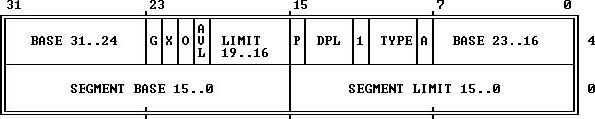
\includegraphics[width=0.8\textwidth]{figures/SegmentDescriptorStructure.png}
    \caption{段描述符结构}
    \label{fig:SegmentDescriptorStructure}
\end{figure}

通过设置GDT,系统可以在保护模式下实现内存的分段管理和保护,使得不同的程序和任务可以在各自的内存段中独立运行,避免相互干扰,并且增强系统的安全性和稳定性。

\subsubsection{磁盘读取器模块(Disk Reader Module)}

磁盘读取器模块(Disk Reader Module)定义了磁盘操作,使用BIOS中断(INT 0x13)来实现从磁盘读取数据。它包括一个Disk结构体和DiskAddressPacket结构体,用于管理磁盘I/O操作和地址映射。该模块允许从指定的逻辑块地址(LBA)读取多个扇区数据到内存中指定位置。DAP的数据结构定义如\cref{lst:DiskAddressPacketDataStructure}所示,在此不再赘述。

该模块定义了Disk结构体,其中包含用于指定从哪个磁盘块(LBA)开始读取以及数据应加载到内存的哪个位置(buffer)的字段。通过调用init方法,可以对这些字段进行配置,为读取操作做好准备。

read\_sector方法通过配置DiskAddressPacket(DAP),然后使用BIOS中断INT 0x13来从磁盘读取一个扇区的数据。这种方法允许直接与硬件交互,无需操作系统层的支持。该方法的实现与\cref{lst:ReadSectorMethod}相同,在此不再赘述。

read\_sectors方法(\cref{lst:ReadSectorsBootloaderMethod})允许从磁盘连续读取多个扇区。它通过在循环中反复调用read\_sector方法,并逐步将数据加载到目标内存位置,从而实现连续读取。以下是这个函数的实现逻辑:

\begin{enumerate}
    \item \textbf{初始化}:方法初始化两个关键变量:sectors\_left 用于跟踪还需读取的扇区数,而 current\_target 标记了数据应当被复制到的内存起始地址。循环将持续进行,直到所有扇区都被读取完毕。
    \item \textbf{扇区读取}:每次循环迭代,首先通过 read\_sector 方法从磁盘读取单个扇区到缓冲区。接下来,通过内部循环,将缓冲区中的数据逐字节复制到目标内存地址。这一过程涉及到寄存器操作和内联汇编,确保数据正确地从源头移动到目标位置。
          \begin{enumerate}
              \item \textbf{读取字节的汇编代码}:这条汇编指令负责从由 byte\_address 指向的内存位置读取单个字节的数据。byte\_address 是一个寄存器,它包含了要读取数据的具体内存地址。\texttt{mov {0}, [{1:e}]} 的指令格式表示将位于内存地址 \texttt{[{1:e}]}(由 byte\_address 指定)的数据移动到 byte 寄存器中。这里的 byte 作为输出寄存器,用于存储读取的数据,以便后续操作可以使用这个数据。
              \item \textbf{写入字节的汇编代码}:这条汇编指令用于将先前读取并存储在 byte 寄存器中的字节数据写入到由 current\_target 寄存器指定的内存地址中。\texttt{mov [{0:e}], {1}} 的指令格式将 byte 寄存器中的数据移动到 current\_target 指定的内存位置。在这个过程中,current\_target 寄存器作为输入,提供目标地址,而 byte 寄存器则提供要写入的数据。这种方式确保了数据能够被正确地从源位置传输到目标位置,实现数据在内存中的精确控制和布局。
          \end{enumerate}
    \item \textbf{状态更新}:在每次完成单个扇区的读取和复制后,更新磁盘读取位置 self.lba 和剩余扇区计数 sectors\_left。
\end{enumerate}

\begin{listing}[htbp]
    \begin{minted}{rust}
pub fn read_sectors(&mut self, sectors: u16, target: u32) {
    let mut sectors_left = sectors;
    let mut current_target = target;
    while sectors_left > 0 {
        self.read_sector();
        let mut byte_address = self.buffer;
        for _byte_index in 0..SECTOR_SIZE {
            unsafe {
                let mut byte: u8;
                core::arch::asm!("mov {0}, [{1:e}]", out(reg_byte) byte, in(reg) byte_address);
                core::arch::asm!("mov [{0:e}], {1}", in(reg) current_target, in(reg_byte) byte);
            }
            current_target += 1;
            byte_address += 1;
        }
        self.lba += 1;
        sectors_left -= 1;
    }
}
    \end{minted}
    \caption{\texttt{read\_sectors(sectors: u16, target: u32)}方法}\label{lst:ReadSectorsBootloaderMethod}
\end{listing}

\subsubsection{全局描述符表模块(GDT Module)}

全局描述符表模块(GDT Module)包含设置全局描述符表(Global Descriptor Table, GDT)的功能,这是进入保护模式所必需的。描述符表告诉CPU如何处理内存的不同段。全局描述符表(GDT)是一个数据结构,它告诉 CPU 各个内存段的基地址、大小、权限和其他属性。在 MinmusOS 中使用的是平坦内存模型,这意味着整个 4GB 的内存空间被视为一个连续的内存区块,而不是被分割成多个独立的段。

尽管 MinmusOS 使用平坦内存模型,其 GDT 实际上包含三个条目:

\begin{enumerate}
    \item \textbf{第一个条目(空描述符)}:在任何 GDT 中,第一个条目总是被设置为零。这是一个空描述符,不用于任何内存段的访问,但其存在是为了符合 Intel 处理器的要求,该处理器规定 GDT 的第一个条目必须是无效的。
    \item \textbf{第二个条目(代码段描述符)}:这个条目定义了一个代码段,其基址设为 0x0,限制设为 0xFFFF,并且粒度位被设置为 1。粒度位为 1 表示段限制以 4KB 为单位计量,而 0xFFFF 的限制在这种设置下允许访问全部 4GB 的内存空间(因为 0xFFFF * 4KB = 4GB)。代码段的设置允许 CPU 执行存储在其中的代码。
    \item \textbf{第三个条目(数据段描述符)}:与代码段类似,数据段也设定了基址为 0x0 和相同的限制,意味着数据段也覆盖整个 4GB 的地址空间。数据段用于定义普通内存操作的访问权限,如读写数据等。
\end{enumerate}

使用平坦内存模型的主要优点是简化了内存管理。在此模型下,所有程序都使用相同的内存地址映射,这消除了段间切换的开销并简化了程序编写。只要有适当的权限所有的内存都可以被任何执行代码访问,这在多任务操作系统中特别有用,因为它允许简单有效地进行任务切换。

\cref{{lst:GlobalDescriptorTable}}通过定义和设置 GDT 条目来配置操作系统的内存段属性,涵盖了内存段的存在状态、类型、权限、大小以及其他关键属性,确保操作系统在保护模式下能够有效地管理内存访问。

\begin{listing}[htbp]
    \begin{minted}{rust}
pub static GDT: GlobalDescriptorTable = {
    let limit: u64 = {                    // 定义段限制大小(0xFFFF 表示所有 32 位内存)
        let limit_low: u64 = 0xFFFF << 0; // 低位部分,直接设置为 0xFFFF
        let limit_high: u64 = 0xF << 48;  // 高位部分,向左移 48 位
        limit_low | limit_high            // 将低位和高位合并,形成完整的段限制大小,覆盖全部 4GB 内存
    };
    
    let base: u64 = {                     // 定义基址
        let base_low: u64 = 0x0000 << 16; // 基址低位,向左移 16 位
        let base_high: u64 = 0x00 << 56;  // 基址高位,向左移 56 位
        base_low | base_high              // 将低位和高位合并,形成完整的基址,从 0 开始
    };

    let access: u64 = {                   // 定义访问字节
        let p: u64 = 0b1 << 47;           // Present 位,必须为 1,表示内存段是存在的
        let dpl: u64 = 0b00 << 46;        // 描述符特权级别,0 是最高特权级别
        let s: u64 = 0b1 << 44;           // 描述符类型位,标记为代码段或数据段
        let e: u64 = 0b0 << 43;           // 可执行位,标记为非执行,用于数据段
        let dc: u64 = 0b0 << 42;          // 方向位 / 一致位,不适用于数据段
        let rw: u64 = 0b1 << 41;          // 可读可写位,数据段可写,代码段可读
        let a: u64 = 0b0 << 40;           // 访问位,用于跟踪段是否被访问过
        p | dpl | s | e | dc | rw | a     // 合并所有位,设置访问权限和段类型
    };

    let flags: u64 = {                    // 定义标志位
        let g: u64 = 0b1 << 55;           // 粒度标志,设为 1 表示段限制以 4KB 为单位
        let db: u64 = 0b1 << 54;          // 操作数大小,设为 1 表示 32 位操作
        let l: u64 = 0b0 << 53;           // 长模式标志,对于非 64 位代码不设定
        let r: u64 = 0b0 << 52;           // 保留位,未使用
        g | db | l | r                    // 合并标志位,确定段的属性
    };

    let executable: u64 = 0b1 << 43;      // 定义可执行位,专用于代码段,使代码段为可执行

    let zero = GdtEntry {                 // 定义第一个条目(空描述符)
        entry: 0
    };

    let code = GdtEntry {                 // 定义第二个条目(代码段描述符)
        entry: limit | base | access | flags | executable
    };

    let data = GdtEntry {                 // 定义第三个条目(数据段描述符)
        entry: limit | base | access | flags
    };

    GlobalDescriptorTable {               // 定义全局描述符表
        entries: [zero, code, data]
    }
};
    \end{minted}
    \caption{定义全局描述符表}\label{lst:GlobalDescriptorTable}
\end{listing}

在MinmusOS中,全局描述符表(GDT)的管理涉及三个核心的数据结构:\texttt{GdtEntry}(\cref{lst:GdtEntryDataStructure})、\texttt{GdtDescriptor}(\cref{lst:GdtDescriptorDataStructure})和\texttt{GlobalDescriptorTable}(\cref{lst:GlobalDescriptorTableDataStructure})。这些结构体是操作系统与硬件之间沟通如何处理内存段的桥梁。下面详细介绍这些数据结构的作用与实现。

\paragraph{\texttt{GdtEntry} 数据结构}

GdtEntry 结构体表示全局描述符表中的一个条目。在 GDT 中,每个条目(或称为段描述符)定义了一个内存段的基址、限制、访问权限等属性。此结构体的字段 entry 是一个 64 位的整数,包含了段的所有描述信息,按照 x86 架构的段描述符格式编码。使用 \texttt{\#[repr(C, packed)]} 确保结构体没有任何内存对齐填充,与硬件要求的内存布局严格一致。\texttt{\#[derive(Copy, Clone, Debug)]} 在 Rust 中自动为类型实现 Copy、Clone 和 Debug trait\footnote{在 Rust 语言中,trait 是一种定义和共享接口或行为的机制,类似于其他编程语言中的接口(如 Java 的接口)或抽象基类。它允许程序员规定具有哪些方法的类型可以做什么,而不必关心这些方法是如何实现的。这样做可以确保不同的数据类型可以共用一套功能,提高代码的复用性和灵活性。},以支持类型的无缝复制、克隆和调试格式化输出。

\begin{listing}[htbp]
    \begin{minted}{rust}
#[derive(Copy, Clone, Debug)]
#[repr(C, packed)]
pub struct GdtEntry {
    entry: u64,
}
    \end{minted}
    \caption{\texttt{GdtEntry}数据结构定义}\label{lst:GdtEntryDataStructure}
\end{listing}

\paragraph{\texttt{GdtDescriptor} 数据结构}

GdtDescriptor 结构体用于在使用 lgdt 指令加载 GDT 时,向处理器提供 GDT 的大小和内存地址。size 字段存储的是 GDT 的字节大小减去一(因为 GDT 的界限是从零开始计数的)。offset 是一个指向 GlobalDescriptorTable 的指针,表示 GDT 在内存中的位置。

\begin{listing}[htbp]
    \begin{minted}{rust}
pub struct GdtDescriptor {
    size: u16,
    offset: *const GlobalDescriptorTable,
}
    \end{minted}
    \caption{\texttt{GdtDescriptor}数据结构定义}\label{lst:GdtDescriptorDataStructure}
\end{listing}

\paragraph{\texttt{GlobalDescriptorTable} 数据结构}

GlobalDescriptorTable 结构体包含一个固定大小的 GdtEntry 数组,即实际的 GDT,存储着所有的段描述符。提供 load 方法,用于加载 GDT 到 CPU。此方法创建一个 GdtDescriptor 实例,设置 GDT 的大小和地址,然后通过 lgdt 指令告诉 CPU 新的 GDT 的位置。使用 \texttt{\#[repr(C, packed)]} 确保结构体没有任何内存对齐填充,与硬件要求的内存布局严格一致。

\begin{listing}[htbp]
    \begin{minted}{rust}
#[repr(C, packed)]
pub struct GlobalDescriptorTable {
    entries: [GdtEntry; GDT_ENTRIES],
}

impl GlobalDescriptorTable {
    pub fn load(&self) {
        let descriptor = GdtDescriptor {
            size: (GDT_ENTRIES * size_of::<GdtEntry>() - 1) as u16,
            offset: self,
        };
        unsafe {
            core::arch::asm!("lgdt [{0:e}]", in(reg) &descriptor);
        }
    }
}
    \end{minted}
    \caption{\texttt{GlobalDescriptorTable}数据结构定义}\label{lst:GlobalDescriptorTableDataStructure}
\end{listing}

\subsubsection{打印器模块(Printer Module)}

打印器模块(Printer Module)负责输出信息到屏幕。这个模块利用BIOS中断(INT 0x10)来在屏幕上打印字符和字符串。它实现了\texttt{fmt::Write} trait,使得可以使用Rust的格式化宏如\texttt{print!}和\texttt{println!}等来输出格式化文本。

\paragraph{结构体和全局变量}

定义为 \texttt{pub static mut PRINTER: Printer = Printer \{\}},这是一个全局可变的 Printer 实例。它声明为 mut 表示它是可变的。Printer 为一个空结构体,作为方法的容器,用于实现打印功能。

\paragraph{实现 \texttt{fmt::Write} trait}

为 Printer 实现 \texttt{fmt::Write} trait 的 write\_str 方法(如\cref{lst:WriteStrMethod}),允许使用 Rust 的格式化字符串功能。此方法接受一个字符串切片 s 并调用 prints 方法来逐字符打印。成功后返回 \texttt{fmt::Result} 类型的 \texttt{Ok(())}。

\begin{listing}[htbp]
    \begin{minted}{rust}
impl fmt::Write for Printer {
    fn write_str(&mut self, s: &str) -> fmt::Result {
        self.prints(s);
        Ok(())
    }
}
    \end{minted}
    \caption{write\_str方法}\label{lst:WriteStrMethod}
\end{listing}

\paragraph{实现Printer}

Printer提供了三种方法(\cref{lst:PrinterImplementation}),printc 方法用于在屏幕上打印一个字符,prints 方法用于在屏幕上打印一个字符串,clear 方法用于清除屏幕并将显示重置为文本模式。

\begin{enumerate}
    \item \textbf{\texttt{printc} 方法}:printc 方法用于在屏幕上打印一个字符。该方法使用内联汇编代码调用 INT 0x10 BIOS 中断来将字符显示在屏幕上。在这里,al 寄存器同样装载字符的 ASCII 值,ah 寄存器设置为 0x0e 以选择 BIOS 的“显示字符”的功能,bx 寄存器设置为 0 用于选择默认的显示页。这段代码使得 BIOS 根据 al 寄存器的值在屏幕上打印相应的字符。
    \item \textbf{\texttt{prints} 方法}:prints 方法接收一个字符串,并遍历其中的每个字符,使用 printc 方法逐个打印到屏幕。这是通过一个简单的循环实现的,循环遍历字符串的每个字符并将其传递给 printc 方法。这种方法简洁有效地处理了字符串的逐字符显示,适用于在屏幕上输出完整的文本行或消息。
    \item \textbf{\texttt{clear} 方法}:clear 方法用于清除屏幕并将显示重置为文本模式。这是通过调用 INT 0x10 BIOS 中断实现的,其中 ax 寄存器设置为 0x0003。这个特定的中断和 ax 值的组合告诉 BIOS 将视频模式重置到标准文本模式,并清空当前显示的内容。使用这种方法可以快速清除屏幕中的所有文本。
\end{enumerate}

\begin{listing}[htbp]
    \begin{minted}{rust}
impl Printer {
    pub fn printc(&self, c: char) {
        unsafe {
            asm!(
            "int 0x10",
            in("al") c as u8,
            in("ah") 0x0eu8,
            in("bx") 0u16,
            );
        }
    }

    pub fn prints(&self, s: &str) {
        for c in s.chars() {
            self.printc(c);
        }
    }

    #[allow(dead_code)]
    pub fn clear(&self) {
        unsafe {
            asm!("int 0x10", in("ax") 0x0003u16);
        }
    }
}
    \end{minted}
    \caption{Printer实现}\label{lst:PrinterImplementation}
\end{listing}

\paragraph{实现宏}

MinmusOS 实现了三种宏:\texttt{clear!} 宏用于清除屏幕显示,\texttt{print!} 宏提供格式化文本输出到屏幕,而 \texttt{println!} 宏在 \texttt{print!} 的基础上额外添加了自动换行功能。宏实现工具函数见\cref{lst:MacroImplementationUtils}。

\begin{enumerate}
    \item \textbf{\texttt{clear!} 宏}:\texttt{clear!} 宏提供了一个简单而直接的方式来清除屏幕的内容。它的实现包括一条单独的语句,调用内部定义的 \_clear() 函数。这个函数通过执行 Printer 类的 clear 方法来清空屏幕,后者使用 BIOS 中断 INT 0x10 来设置视频模式并清除显示。通过这个宏,开发者可以在任何地方简单地写 \texttt{clear!()}; 来清除屏幕,而不需要直接调用底层清屏函数。
    \item \textbf{\texttt{print!} 宏}:\texttt{print!} 宏允许开发者以类似于 Rust 标准库中的 \texttt{print!} 功能的方式打印格式化文本。这个宏接收任意数量的参数,使用 \texttt{format\_args!} 宏将这些参数转换成一个 \texttt{fmt::Arguments} 类型,这是一个预格式化的文本表示。之后,它调用 \_print 函数,该函数实际上通过 write\_fmt 方法将文本输出到屏幕。这使得打印操作不仅支持简单的字符串,还支持复杂的格式化操作。
    \item \textbf{\texttt{println!} 宏}:\texttt{println!} 宏扩展了 \texttt{print!} 宏的功能,添加了自动换行的特性。它在功能上类似于 \texttt{print!} 宏,但在每次调用结束时自动加上换行符。这个宏同样使用 \texttt{format\_args!} 来处理输入的参数并格式化它们,然后调用 \_print 来输出最终的字符串。\texttt{println!} 宏非常适合用于输出日志信息或其他需要按行处理的文本输出,简化了每次输出后手动添加换行符的需要。
\end{enumerate}

\begin{listing}[htbp]
    \begin{minted}{rust}
pub fn _print(args: fmt::Arguments) {
    use core::fmt::Write;
    unsafe {
        PRINTER.write_fmt(args).unwrap();
    }
}

pub fn _clear() {
    unsafe {
        PRINTER.clear();
    }
}
    \end{minted}
    \caption{宏实现工具函数}\label{lst:MacroImplementationUtils}
\end{listing}

\subsubsection{主启动程序(Main Boot Program)}

主启动程序是引导加载器的入口点。它负责初始化硬件设备、设置内存模式、加载内核到内存,并转交控制权到内核。此模块包含了转换到不真实模式和保护模式的逻辑,以及核心启动逻辑。

错误处理函数 \texttt{fail} 和紧急停止处理函数 \texttt{panic} 的实现和\cref{sec:MainBootProgram}类似,在此不再赘述。

\paragraph{常量定义}

\cref{lst:ConstantDefinitions}定义了内核数据的存放位置和大小,以及内存中的目标位置。

\begin{listing}[htbp]
    \begin{minted}{rust}
const KERNEL_LBA: u64 = 4096;          // 内核的逻辑块地址(LBA)
const KERNEL_SIZE: u16 = 2048;         // 内核大小,以扇区为单位
const KERNEL_BUFFER: u16 = 0xBE00;     // 用于复制内核的缓冲区的内存地址
const KERNEL_TARGET: u32 = 0x00100000; // 内核被加载到内存中的目标地址
    \end{minted}
    \caption{常量定义}\label{lst:ConstantDefinitions}
\end{listing}

\paragraph{切换到不真实模式(Unreal Mode)}

unreal\_mode 函数(\cref{lst:UnrealModeMethod})主要是用来设置处理器从实模式(Real Mode)切换到所谓的“Unreal Mode”,代码实现逻辑如下:

\begin{listing}[htbp]
    \begin{minted}{rust}
fn unreal_mode() {
    // 保存段寄存器值
    let ds: u16;
    let ss: u16;
    unsafe {
        asm!("mov {0:x}, ds", out(reg) ds);
        asm!("mov {0:x}, ss", out(reg) ss);
    }

    // 加载全局描述符表(GDT)
    GDT.load();

    unsafe {
        // 读取并修改 CR0 寄存器
        let mut cr0: u32;
        asm!("mov {0:e}, cr0", out(reg) cr0);
        let cr0_protected = cr0 | 1;
        asm!("mov cr0, {0:e}", in(reg) cr0_protected);

        // 设置新的段寄存器值
        asm!("mov {0:x}, 0x10", "mov ds, {0:x}", "mov ss, {0:x}", out(reg) _);

        // 恢复 CR0 和段寄存器
        asm!("mov cr0, {0:e}", in(reg) cr0);
        asm!("mov ds, {0:x}", in(reg) ds);
        asm!("mov ss, {0:x}", in(reg) ss);
    }
}
    \end{minted}
    \caption{切换到不真实模式(Unreal Mode)实现}\label{lst:UnrealModeMethod}
\end{listing}

\begin{enumerate}
    \item \textbf{保存段寄存器值}:通过内联汇编命令保存当前的数据段寄存器(DS)和栈段寄存器(SS)。这是为了后面能够恢复这些寄存器的原始值,确保在修改后可以返回到原始状态。
    \item \textbf{加载全局描述符表(GDT)}:调用加载全局描述符表,GDT 中定义了不同的内存段,包括其大小、权限等信息。加载 GDT 是为了使得后续可以设置更大的段限制。
    \item \textbf{读取并修改 CR0 寄存器}:首先读取 CR0 寄存器的当前值,然后设置最低位(启用保护模式的标志位)。
    \item \textbf{设置新的段寄存器值}:将段寄存器 DS 和 SS 设置为 GDT 中新的段选择子(0x10),这指向一个具有更大段限制的描述符。
    \item \textbf{恢复 CR0 和段寄存器}:最后,将 CR0 寄存器恢复到原来的值,并将 DS 和 SS 段寄存器恢复到之前保存的值。这是为了确保系统的稳定性和正确回到原始状态。
\end{enumerate}

Unreal Mode 的主要功能是允许实模式下的应用程序访问更大的内存空间。虽然 CPU 仍然在实模式下运行,但通过修改段寄存器的限制,可以访问高于 1MB 的内存。这在早期的 DOS 扩展中非常有用,允许 16 位程序突破 640KB 内存限制。在现代操作系统开发中,这种模式可以在启动过程中用于设置和初始化更复杂的内存管理机制。

\paragraph{切换到保护模式(Protected Mode)}

protected\_mode 函数(\cref{lst:ProtectedModeMethod})实现了在一个操作系统的启动过程中从实模式切换到保护模式。保护模式是现代操作系统中使用的模式,它支持更高级的特性,如更大的内存寻址、虚拟内存和进程隔离等。代码实现逻辑如下:

\begin{enumerate}
    \item \textbf{设置 CR0 寄存器以启用保护模式}
          \begin{enumerate}
              \item \texttt{mov eax, cr0}:将控制寄存器 CR0 的值移动到 EAX 寄存器中。CR0 寄存器中的位控制着处理器的操作模式和状态。
              \item \texttt{or al, 1}:将 EAX 寄存器的最低字节 AL 与 1 进行逻辑或操作,这样设置了 CR0 寄存器的最低位(PE 位,Protection Enable),用以启动保护模式。
              \item \texttt{mov cr0, eax}:将修改后的 EAX 寄存器的值回写到 CR0 寄存器,从而实际启用保护模式。
          \end{enumerate}
    \item \textbf{推送内核入口地址}:这一步将内核的目标入口地址推送到栈上。这个地址稍后将用于跳转到内核执行。
    \item \textbf{长跳转以刷新管线和真正切换到保护模式}:执行一个长跳转,这里的 \texttt{\$0x8} 是新的代码段选择子,指向 GDT 中定义的保护模式代码段。\texttt{\$2f} 是标签,跳转到下一行代码,这种跳转是必需的,因为它使 CPU 的内部管线刷新,确认从实模式完全切换到保护模式。
    \item \textbf{设置段寄存器和跳转到内核}
          \begin{enumerate}
              \item \texttt{.code32}:指示开始使用 32 位代码。
              \item \texttt{mov {0:e}, 0x10}:设置各个段寄存器指向 GDT 中的相应保护模式段。
              \item \texttt{mov ds, {0:e}}、\texttt{mov es, {0:e}}、\texttt{mov ss, {0:e}}:分别将数据段、附加段和栈段寄存器设置为保护模式下的值。
              \item \texttt{pop {1:e}}:从栈中弹出之前保存的内核入口地址。
              \item \texttt{call {1:e}}:跳转到内核的入口地址开始执行内核代码。
          \end{enumerate}
\end{enumerate}

\begin{listing}[htbp]
    \begin{minted}{rust}
fn protected_mode() {
    unsafe {
        // 设置 CR0 寄存器以启用保护模式
        asm!("mov eax, cr0", "or al, 1", "mov cr0, eax");

        // 推送内核入口地址
        asm!("push {0:e}", in(reg) KERNEL_TARGET);

        // 长跳转以刷新管线和真正切换到保护模式
        asm!("ljmp $0x8, $2f", "2:", options(att_syntax));

        // 设置段寄存器和跳转到内核
        asm!(
        ".code32",
        "mov {0:e}, 0x10",
        "mov ds, {0:e}",
        "mov es, {0:e}",
        "mov ss, {0:e}",
        "pop {1:e}",
        "call {1:e}",
        out(reg) _,
        in(reg) KERNEL_TARGET,
        );
    }
}
    \end{minted}
    \caption{切换到保护模式(Protected Mode)实现}\label{lst:ProtectedModeMethod}
\end{listing}

\paragraph{主入口函数}

\cref{lst:BootloaderMainFunction}定义了一个操作系统引导加载器中的主入口函数 \_start。这个函数是操作系统从实模式到保护模式转换过程中的关键部分,并且负责加载内核到内存中。下面是对该函数中各部分的解释:

\begin{listing}[htbp]
    \begin{minted}{rust}
#[no_mangle]
#[link_section = ".start"]
pub extern "C" fn _start() -> ! {
    println!("[INFO] Switching to Unreal Mode...");
    unreal_mode();
    println!("[INFO] Loading Kernel...");
    unsafe {
        DISK.init(KERNEL_LBA, KERNEL_BUFFER);
        DISK.read_sectors(KERNEL_SIZE, KERNEL_TARGET);
    }
    println!("[INFO] Loading Global Descriptor Table...");
    GDT.load();
    println!("[INFO] Switching to Protected Mode...");
    protected_mode();
    loop {}
}
    \end{minted}
    \caption{主入口函数}\label{lst:BootloaderMainFunction}
\end{listing}

\begin{enumerate}
    \item \textbf{\texttt{\#[no\_mangle]}}:这个属性防止 Rust 编译器改变这个函数的名称,这是确保启动代码能正确链接到这一特定入口点非常重要的一步。
    \item \textbf{\texttt{\#[link\_section = ".start"]}}:指示编译器将这个函数放在 ELF 文件\footnote{ELF(Executable and Linkable Format)文件格式是一种广泛使用的标准文件格式,用于定义可执行文件、对象代码、共享库和核心转储。这种格式主要在Unix和Unix-like系统(如Linux、Solaris、IRIX、FreeBSD、NetBSD等)中使用,但也可在其他操作系统上实现。ELF 文件的主要用途包括可执行文件、对象文件、共享库、核心转储文件等。ELF 格式提供了一种灵活且强大的方式来组织和使用不同类型的代码和数据。这种格式的统一性和广泛支持使其成为了现代操作系统在处理可执行文件和库时的首选格式。它也支持高级特性如动态链接和执行时重定位,这些特性对于现代操作系统的动态性和模块化非常重要。}的 .start 段中。这是 bootloader 约定用于存放入口点代码的段。
    \item \textbf{切换到 Unreal Mode}:调用 unreal\_mode 函数,这个函数设置处理器以允许访问扩展的内存空间,虽然仍然在 16 位模式下运行。
    \item \textbf{加载内核}:在 unsafe 块中,调用 \texttt{DISK.init()} 和 \texttt{DISK.read\_sectors()} 来初始化磁盘并从磁盘读取内核到内存中的指定位置。这需要使用 unsafe 语句,因为它涉及直接的硬件操作和内存操作,这些操作可能导致未定义行为。
    \item \textbf{加载全局描述符表(GDT)}:调用 \texttt{GDT.load()} 函数来设置 CPU 的段描述符,这是进入保护模式前必需的步骤。
    \item \textbf{切换到 Protected Mode}:调用 \texttt{protected\_mode()} 函数,该函数负责将 CPU 从 Unreal Mode 完全切换到 32 位的保护模式。此模式支持更高级的内存管理和保护功能。
    \item \textbf{无限循环}:\texttt{loop \{\}}确保 \_start 函数在执行完成后不会返回或执行任何其他未定义的操作。
\end{enumerate}

\subsubsection{链接器脚本(Linker Script)}

这个链接器脚本(\cref{lst:BootloaderLinkerScript})专为操作系统的引导程序设计,目的是定义和控制引导程序在内存中的布局。链接器脚本在系统启动过程中起到至关重要的作用,确保引导程序正确地加载和执行。脚本总体可以分为以下几个关键部分来概括其作用:

\begin{enumerate}
    \item \textbf{程序入口点}:指定 \_start 函数为程序的入口点,这是系统开始执行引导程序的地方。
    \item \textbf{段的配置}:设置引导程序的加载地址。0x7C00 是 BIOS 传统上将引导扇区加载到内存的位置,加上 512 字节(一个扇区的大小)是为了紧接引导扇区之后开始。
    \item \textbf{各种内存段的定义}:.start 包含引导程序的实际入口代码,.text 包含程序的机器代码,.bss 用于存储程序中未初始化的数据,.rodata 包含只读数据,.data 包含已初始化的全局变量和静态变量,.eh\_frame 和 .eh\_frame\_hdr 包含用于支持运行时错误处理的异常处理信息。
    \item \textbf{内存布局的结束配置}:将位置指针设置为引导加载器起始位置加上 32KB 减 2 字节,确保引导加载器的大小正好为 32KB。在内存中设置一个结束标记(使用 \texttt{SHORT(0XDEAD)}),用于标识引导加载器的结束。
\end{enumerate}

\begin{listing}[htbp]
    \begin{minted}{text}
/* 配置程序入口点 */
ENTRY(_start)

/* 配置段的顺序和位置 */
SECTIONS {
    /* 配置引导加载器的开始地址为 0x7C00 加 512B(即一个扇区后),这是 BIOS 启动扇区的传统位置 */
    . = 0X7C00 + 512;
    _bootloader_start = .;

    /* 定义启动段,包含启动代码的实际入口点 */
    .start : {
        *(.start)
    }

    /* 定义代码段,包含程序的机器代码 */
    .text : {
        *(.text .text.*)
    }

    /* 定义 BSS 段,包含程序中未初始化的数据 */
    .bss : {
        *(.bss .bss.*)
    }

    /* 定义只读数据段,包含常量等不应被程序修改的数据 */
    .rodata : {
        *(.rodata .rodata.*)
    }

    /* 定义数据段,包含已初始化的全局变量和静态变量 */
    .data : {
        *(.data .data.*)
    }

    /* 配置异常处理信息,用于支持运行时错误处理 */
    .eh_frame : {
        *(.eh_frame .eh_frame.*)
    }
    .eh_frame_hdr : {
        *(.eh_frame_hdr .eh_frame_hdr.*)
    }

    /* 将位置指针设置为引导加载器起始位置加上 32KB 减 2B,确保引导加载器大小为 32KB */
    . = _bootloader_start + 0X8000 - 2;

    /* 在内存中设置一个结束标记,用于标识引导加载器的结束 */
    .end_marker :
    {
        SHORT(0XDEAD)
    }
}
    \end{minted}
    \caption{bootloader/linker.ld}\label{lst:BootloaderLinkerScript}
\end{listing}

在 Rust 项目中,build.rs 文件充当构建脚本的角色,主要用于在项目编译前执行自定义的构建任务。构建脚本的实现与\cref{LinkerScript}相同,在此不再赘述。

通过精确地控制各个内存段的位置和大小,这个脚本确保引导程序能够被正确地加载到预期的内存地址,并且所有的代码和数据都按预期方式进行组织。通过配置 .eh\_frame 和 .eh\_frame\_hdr,增强了程序的健壮性,使得在出现运行时错误时能够进行有效的异常处理。

至此我们实现了从实模式到保护模式的切换,并完成了内核的加载(\cref{fig:BootloaderPresentation})。

\begin{figure}[htbp]
    \centering
    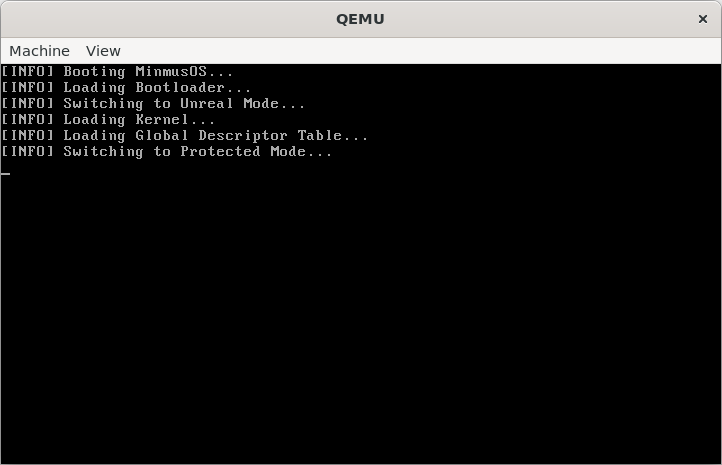
\includegraphics[width=0.8\textwidth]{figures/BootloaderPresentation.png}
    \caption{引导加载器演示}
    \label{fig:BootloaderPresentation}
\end{figure}